\chapter{Background}

%5 pages minimum!, hopefully 8-10 though doubt it

%Section 1 on neural networks and how they work, CNNs, Alexnet, Inception (but no further)
\section{Neural networks}

%3-4 sentences before figure, leading into the topic "since ancient times" sort of talk?

Neural networks are something everyone has, even if they do not understand the concept. 
Neurons in our brains transmit signals to other neurons, which in turn do the same to the next neurons in line. 
Some neurons are connected to many neurons, while other neurons may only be connected to a few. 
Through their connections, the neurons are creating all sorts of connection shapes ranging from massive trees to a short loop. 
Throughout a lifetime, these connections change as the brain learns and forgets information.

%figure of typical nn
\begin{figure}[htbp]  % order of priority: h here, t top, b bottom, p page
  \centering
  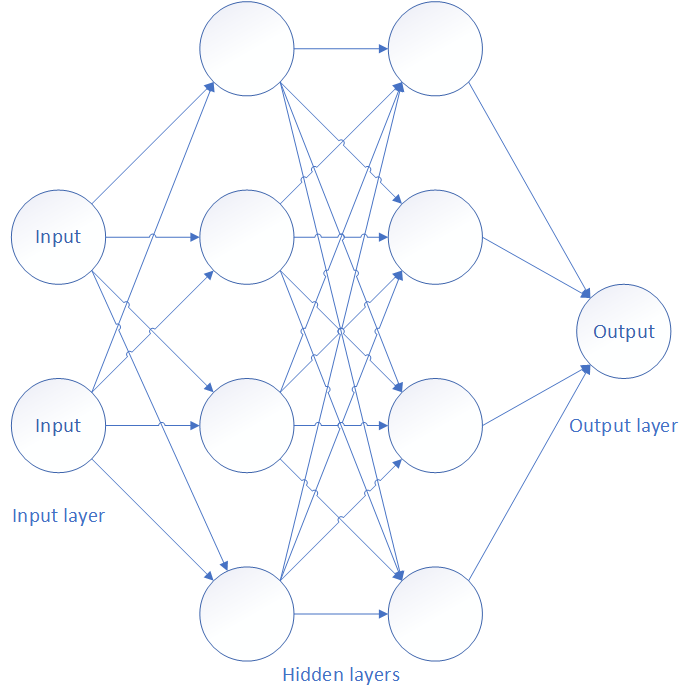
\includegraphics[width=.6\textwidth]{figures/small_model.png}
  \caption{Illustration of a simple feed-forward neural network}
  \label{fig:simplenn}
\end{figure}

%3-6 sentences after figure explaining the basic concept of a nn

In computing, standard simple neural networks are clearly defined into layers, with a clear point of entry called the "input" layer, with the result coming out of the "output" layer. 
A basic illustration of this is provided in \cref{fig:simplenn}. 
Information we want to be processed into the output result is inserted into each of its designated input neurons. 
Between the input and output layers, we can place one or more hidden layers.
These hidden layers abstract the input from the output, allowing the network more flexibility in making connections between input and output. 
In the case of \cref{fig:simplenn}, the input could be the current weekday and the time of day, with the output being a value between 0 and 1 determining if it is time to eat dinner. 
On weekdays it could say that between 18:00 and 19:00 is the best time to eat dinner, while during the weekend it could extend the time to be sooner or later.

%General theory for what a neural network is
%source to wikipedia here?
%Small figure showing what it looks like (simple neuron image thing)

\subsection{History}

%Rundown on nn history, 4 paragraphs
%p1: Early history, Hebb, backpropagation Werbos 1975

History of artificial neural networks used in computing can be traced back to its common roots with medicine and psychology that the NNs attempt to mimic. 
Towards the late 1940s, Donald Hebb \cite{hebb2005organization} described a theory of how cells in a brain function together. 
As the brain cells fire electrical signals to other cells, those connections are strengthened and happen more frequently.
Artificial neural networks use this theory loosely to translate the signal received in the input neurons into proper outputs.
While the Hebbian theory allowed for the creation of first neural networks, these networks were not very useful due to limitations in computing power and lack of more complex structures. 
The creation of deep neural networks with multiple layers was practically impossible until the creation of the backpropagation algorithm in 1975 by Paul Werbos\cite{werbos1975beyond}. 
Backpropagation allows for the errors in the learning process to be sent back through multiple network layers, and adjust all of the weights in the network.


%p2: MOS-VLSI to create a practical network, max-pooling introduced in 1992, 90s-alexnet

Even with the creation of the backpropagation algorithm, the computational power of the time did not allow for very complex neural networks. 
As execution in software was too difficult at the time, hardware solutions were created. Using the recent at the time metal-oxide semiconductors, in 1989, neural networks were implemented using very-large-scale integration in analog, rather than digital\cite{mead2012analog}. 
During the following two decades, various techniques were developed to enable neural networks to handle more complex problems.
Among others, max-pooling was introduced in 1992\cite{cresceptron1992}, and continuous improvement of existing and new technologies enabled neural networks to grow in relevance as more powerful hardware became available.

%p3: alexnet, non-commercial?, illustration of alexnet

The first in the series of convolutional neural networks that drastically improved the field of Artificial Intelligence is the deep neural network by Alex Krizhevsky \cite{Krizhevsky:2017:ICD:3098997.3065386}, created in 2012. 
%Deep layer technique, many layers stacked on top
A neural network becomes "deep" when more than one layer is placed between the input and output layer.
AlexNet was constructed with five convolutional layers, followed by three dense layers, of which the last dense layer was the output layer.
Also, several max-pooling layers were placed throughout the model.
By using multiple convolutional layers in sequence, AlexNet managed to beat all of its competition that year in the ImageNet\cite{ImageNetMain} challenge\cite{ImageNet2012}.


%p4: googlenet, commercial entity behind

After this breakthrough, commercial entities like Google used the findings in this paper to create the Inception\cite{szegedy2014going} network. 
This network utilized a combination of different convolutional layers in what it calls the Inception Module, seen in figure \cref{fig:inception}.
Unlike the previous models where the next layer strictly followed one layer, the Inception network has one-to-many and many-to-one connections that enable it to do multiple different operations on input from the same previous layer.
By combining the layers into building blocks, and then stacking them on top of each other, the first Inception NN beat out its competition in the 2014 challenge\cite{ImageNet2014}. %1-2 more sentences in the middle of this block
%


\begin{figure}[htbp]  % order of priority: h here, t top, b bottom, p page
  \centering
  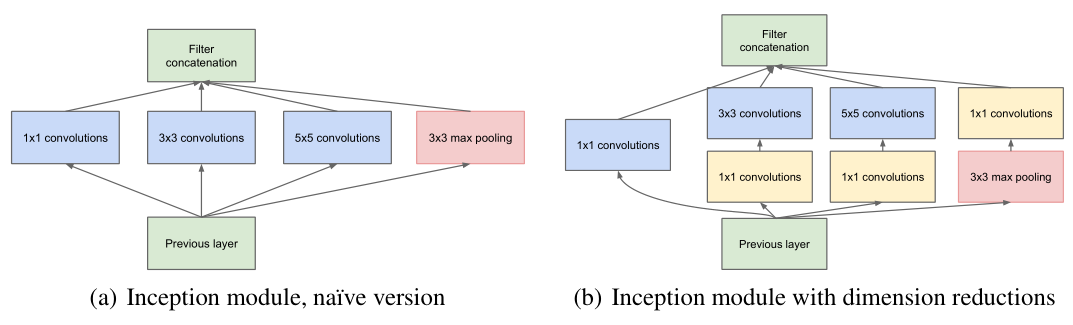
\includegraphics[width=.7\textwidth]{figures/google2.PNG}
  \caption{The Inception Module\cite{szegedy2014going}, without (left) and with (right) pooling layers in the module.}
  \label{fig:inception}
\end{figure}

\subsection{Convolutional neural networks}

While a neural network like the one shown in \cref{fig:simplenn} can be used to receive some results for simple data with no structure in the input, extracting information from sound and images requires the network to understand the relationship between each input. 
For the network to learn the meaning of the input structure, several different types of layers are mixed, each applying its specific operation to the input it receives.


%Rundown on what a CNN is, what it is used for
%Subsections for the direct explanation on the layers

%6-8 sentences, explain basics
%1-2 links to more on this?

%S0: dense layers, basic
\subsubsection{Dense layer}
%4-6 sentences, explain what it is and where it's placed, FIGURE
The dense layer is the simplest of all layers in all neural networks.
Looking back at \cref{fig:simplenn}, the hidden layer in the figure is a dense layer.
A dense layer only applies a simple multiplication operation on the input it receives with the weights of the connections between the neurons.
In convolutional neural networks, this layer is usually placed at the end of the network to represent the features that the previous layer has learned to detect.



%S1: conv layer (in particular the 1D version)
\subsubsection{Convolutional layer}
%8-12 sentences, core of the network, FIGURE
%What a conv layer is, the operation, go in detail on the 1D network
The convolutional layer is the central part of the convolutional neural network.
Unlike the dense layer that applies only a simple multiplication operation, this layer applies a filter over multiple inputs next to each other. 
This filter is can also be called the convolution window or the kernel.
The filter applies a multiplication operation to every item in the convolution window and then sums all of the results into one number.
An example of the thesis relevant 1D convolution operation can be seen in \cref{fig:conv_example}.

\begin{figure}[htbp]  % order of priority: h here, t top, b bottom, p page
  \centering
  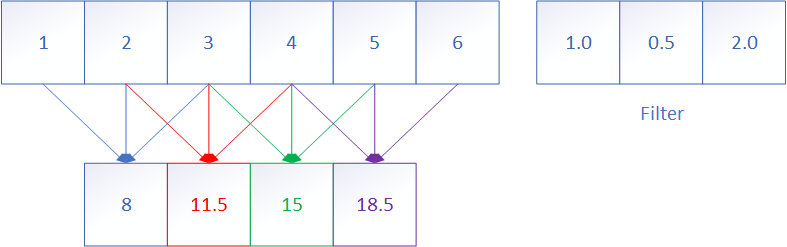
\includegraphics[width=.9\textwidth]{figures/conv_op.png}
  \caption{Example of a convolution operation. Padding operations on the borders not included.}
  \label{fig:conv_example}
\end{figure}

In a convolutional layer, there can be any number of filters, and each of these filters can be different to produce different results from the same data.
By combining these different filters, the model can be trained to detect different features in the input data, combinations of which can represent different output classes.


%S2: pooling layers, max and average
\subsubsection{Pooling layer}
%8-12 sentences, max and average pooling layer, FIGURE
%Explain the concept, what the pooling layer is
The pooling layer is a normal part of the complete convolutional neural network.
Whether one processes audio or images, the input is often an extensive matrix, while the output is often at most 1000 classes, as is the case with the AlexNet\cite{Krizhevsky:2017:ICD:3098997.3065386} and Inception\cite{szegedy2014going} networks.
Since suddenly reducing the matrix down to only 1000 neurons or less would wash out the significance of every single feature detected by the network, pooling layers are applied to reduce the size of the input gradually throughout the network.
For this thesis, two different pooling layers have been considered, the max-pooling layer and the average pooling layer.
All pooling layers apply a filter similar to the convolution window on the input data.
Unlike convolution, in the case of the max pooling operation, the highest value in the window is passed to the next layer.
The average pooling layer, on the other hand, calculates the average value in the filter and passes this forward.
In addition to doing this, the size of the network is commonly divided by the size of the filter.
As shown in \cref{fig:poolexample}, the input in both pooling types is reduced from 6 values down to 3 in the next layer.
While this is common, it is not strictly necessary and can be adjusted freely.


\begin{figure}
    \centering
    \begin{subfigure}[b]{.45\textwidth}
        \centering
        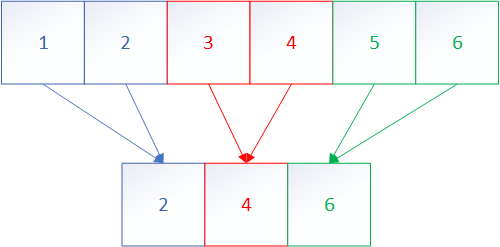
\includegraphics[width=\textwidth]{figures/maxpooling.png}
        \caption{Max pooling}
        \label{sfig:maxpoolexample}
    \end{subfigure}
    \hfill
    \begin{subfigure}[b]{.45\textwidth}
        \centering
        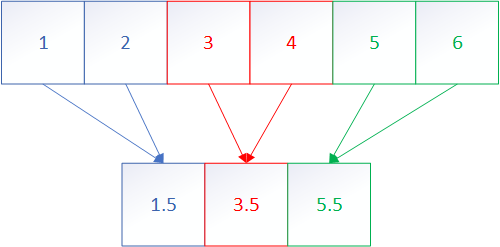
\includegraphics[width=\textwidth]{figures/avgpooling.png}
        \caption{Average pooling}
        \label{sfig:avgpoolexample}
    \end{subfigure}
    \caption{Two examples of the pooling operation on the same initial values}
    \label{fig:poolexample}
\end{figure}

%Custom images for all of this, but based on theory

%One more subsection tied to optimizers, loss functions and other stuff?
%Working title Gradient descent, uncertain if correct
%New title, training the neural network, more precise
\subsection{Training the neural network}
%Network needs to be trained to work, the process of adjusting this is (title of part)
%4-6 sentences to tie in backprop from history, only "part" of the puzzle

Creating the neural network structure is only the first step in the process, as the initial weights in the model are utterly meaningless to the desired result.
As mentioned in the history of neural networks, backpropagation was already figured out in 1975\cite{werbos1975beyond}.
For each training pass over the dataset, also called an epoch, the training process executes several vital steps that can be modified to change the weights more optimally to what is desired.


\subsubsection{Loss functions}
%Categorical crossentropy
%6-8 sentences to explain crossentropy

During the training process, the network predicts a value on the given input, and the expected value is also known.
A loss function is used to calculate the difference between these two values.
When creating a neural network that has to classify the input into different classes, the most commonly used loss function is the categorical cross-entropy loss function\cite{wiki:crossentropy}.
In short, the result of the loss function can be considered the distance between the result predicted by the network and the desired result.
Therefore, to achieve the best possible weight combination in the neural network, the goal is to reduce this number as much as possible.

\subsubsection{Optimizers}
%RMSProp, Adam (and variants), SGD?
%8-10 sentences?

While knowing the loss function number is useful for the human watching the training process, it is the role of the optimizer to take the loss values and turn them into better weights.
Optimizer is another word for the stochastic gradient descent algorithm\cite{wiki:sgd}, of which there exist many variations.
The optimizer takes the loss value from each sample and calculates the most optimal way to reduce the total error by adjusting the weights.
As using the entire dataset can be impossible with sufficiently large datasets, and using single samples can produce local minimums, it is common to pass small batches of several dozen samples per batch to the optimizer.
To ensure that the weights are not changed randomly, all optimizers use a parameter called the learning rate.
The learning rate controls the distance by which each weight can be changed during one training epoch.
While the older SGD optimizer only has one learning rate for the entire operation, newer optimizers like AdaGrad, RMSProp and Adam create an adapted learning rate for each parameter. 
Selective modification of weights allows the optimizers to modify some weights more than others, leaving weights that have little effect on the loss alone while working on the more problematic weights.


\subsubsection{Metrics}
%Loss number, accuracy
%4-6 sentences to explain metrics
Finally, various metrics can be reported by the training program to the user, and be used to stop training early.
In general, the two metrics used to determine how good a neural network is are loss and accuracy.
Loss is the value output by the loss function, and accuracy is the percentage of times the network produced an accurate result.
With the loss, the best value is zero, while with accuracy, the goal is to get as close to one as possible.
As neural networks can be overfitted for a particular dataset, it is common to use a part of the dataset as a validation set.
The goal of the validation set is to also reach as perfect values as possible; however, this dataset is not used during the training process.
By excluding part of the dataset in this manner, the second set of metrics is produced with the validation prefix.
In addition to the standard loss and accuracy metrics, other metrics can be used, like the top-K categorical accuracy.
This variant of the accuracy metrics tracks how often the target value is in the top-K number of targets, rather than tracking how well the actual target was predicted.

\subsection{Transfer learning}
%Why
Once a neural network is trained to do one task, it can often be adapted to do a similar but different task.
This process is called transfer learning\cite{wiki:transferlearning}.
In the case of convolutional neural networks, the earlier layers in the model will often pick up generic features in the data, with the more specific features about the output class coming up towards the end of the model.

%How
As the old model is fit to work on its original task, to start the process of transfer learning, it is necessary to replace the classification head of the model that is being adapted.
The classification head is the last couple of layers of the network, which is, at minimum, the final output layer.
As the weights in the model are already initialized with feature detection, it is necessary to freeze large sections of the network to prevent the model from quickly losing the features in the first few epochs.
Once the model reaches the top accuracy for the new problem, the previously frozen layers can be frozen to fine-tune the model to the new task, training with a reduced learning rate to prevent information loss in the new classification head.
An example of this process can be found on various documentations of software supporting neural network development, like Tensorflow\cite{tensorflow:transferlearning} and Matlab\cite{MatlabPretrained}.


%What the end result is
Assuming that the old and new problem areas allow for transfer learning, the result of transfer learning is a very high-quality neural network model that takes only a fraction of the time to develop.

%Section 2 (probably earlier) on audio sample processing, what mfcc is, librosa
%Working title
\section{Audio processing}
%Necessary things to explain due to being part of MFCC:


%Fourier transform
\subsection{Fourier transform}
As raw audio is not too useful on its own, to make use of the raw audio signal, it is necessary to isolate various parts of the audio into separate parts.
As audio is effectively a lot of sines and cosines combined to form a complex signal, these parts of the signal can be separated to find the frequencies that constitute part of the raw audio.
The process of extracting these frequencies is computed using the Fourier transform.
By extracting each of the signal waves that form the full audio signal, it is possible to analyze how each change over time, identifying the relevant signal waves while also detecting noise in the audio.
The detected noisy signal waves can be removed while preserving the vital signal waves for further processing.


%Mel scale
\subsection{Mel scale}
Humans hear differences in sound on a different scale than the linear scale of the Hertz frequencies.
When the sound is of low frequency, minute differences can be easily detected, while higher frequencies need more significant frequency differences to be found by the human ear.
To more accurately represent the scale of sound heard by the human ear, the Mel scale was introduced in 1937\cite{melpaper}.
By applying the Mel scale to frequency data, the frequencies of the signal can be represented on a more linear scale from the view of a human listener.

%Discrete cosine transform
\subsection{Discrete cosine transform}
A raw audio signal takes much space and is, therefore, essential to compress into smaller, more relevant blocks of information.
Initially developed in the 1970s\cite{dctpaper} for use in image compression, it has also seen much use in audio processing.
Unlike the Fourier transform that operates on both sines and cosines, the DCT operates only on the cosine.
The limitations imposed on the DCT to achieve good compression of the features in raw audio create several assumptions about the input, such as whether the function being transformed is even or odd in the data window being processed.
Because of this, a total of 16 variants of the transform exist, of which half are DCT and the other half are the Discrete sine transforms.
Of these, the most relevant are DCT-2 and DCT-3, which is the inverse of DCT-2, both described in the original paper\cite{dctpaper}.

%Replace title with full name
\subsection{Mel-frequency cepstrum coefficients}
%4-6 sentences describing MFCC
%name combines above to produce analyzable results
Mel-frequency cepstrum is a combination of the above techniques that provide values that are far more analyzable than raw audio.
The process of producing the MFC coefficients from raw audio follows the steps defined

%How to generate (source? no)
\begin{enumerate}
    \item Process the raw audio signal with the Fourier transform
    \item Map the frequencies found in step 1 into the Mel scale
    \item Calculate the log values of each Mel frequency
    \item Process the Mel log values with the Discrete cosine transform
    \item Amplitudes in the spectrum produced by step 4 are the MFCCs
\end{enumerate}

\begin{figure}
    \centering
    \begin{subfigure}[b]{.45\textwidth}
        \centering
        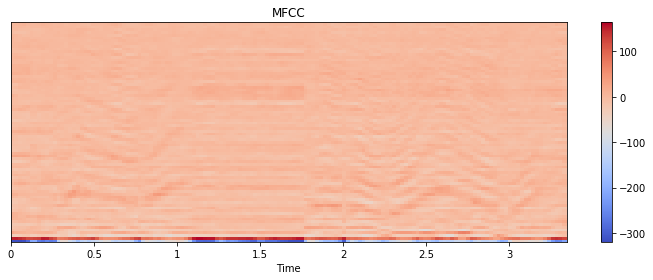
\includegraphics[width=\textwidth]{figures/mfcc2.png}
        \caption{80 MFCCs with DCT-2}
        \label{sfig:mfcc2example}
    \end{subfigure}
    \hfill
    \begin{subfigure}[b]{.45\textwidth}
        \centering
        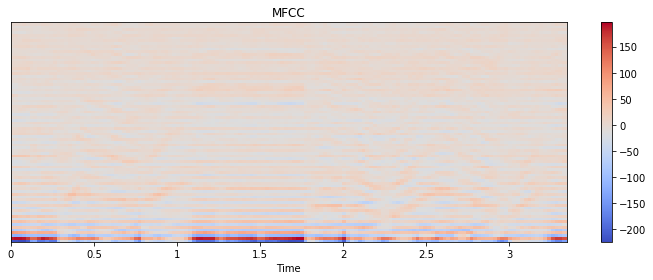
\includegraphics[width=\textwidth]{figures/mfcc3.png}
        \caption{80 MFCCs with DCT-3}
        \label{sfig:mfcc3example}
    \end{subfigure}
    \caption{Two examples of 80 MFCCs generated with DCT-2 and DCT-3 on the same 3.4-second long audio sample}
    \label{fig:mfccexample}
\end{figure}

%figures
%result is stable (20, 40, 80)
It is possible to use different DCTs to generate MFCC values, as presented in \cref{fig:mfccexample}.
One of the benefits of using MFCCs is that the number of coefficients can be scaled as desired.
Should one choose to generate 20, 40, or 80 coefficients for a given sample, the first 20 MFCCs in the 40 and 80 options will match the MFCCs generated in the 20 coefficient option.
In \cref{fig:mfccexample}, a total of 80 coefficents are generated.
Should only 20 MFCCs be needed, the superfluous coefficients can be removed rather than having to generate a new dataset.

%Subsection of MFCC
\subsubsection{MFCC Applications}
%Pull some of the uses for mfcc papers here
%Pull in all of the MFCC application papers that have been found until now, include marine vessels
%Then see if it's enough

One of the recent comparisons between the various audio classification methods has been in grouping audio clips from various entertainment sources into their respective category.
A study conducted in 2011\cite{DHANALAKSHMI2011350} aimed to identify if a particular audio sample originated from music, news, sports, advertisement, cartoon or movie.
This study compared MFCCs to Linear Prediction coefficients and Linear Prediction Derived Cepstrum coefficients.
In the final results of the 2011 study, MFCC has produced superior results when compared to both alternatives, additionally being more superior in helping identify short 1-2 second samples.

Previous students have also used MFCCs at NTNU on similar topics. A former student has used MFCCs to classify audio samples of various marine vessels\cite{marine}.
The audio samples in this project were sonar data generated using a sonar simulation system developed by Kongsberg Defense \& Aerospace.
In this project, a small convolutional neural network using the MFCC variant of the data provided the highest accuracy result.


%Section 3 on trees, current existing methods of grouping data (agg, k-means etc)
%Working title, other can be 
\section{Hierarchical clustering}

%Explain the basics of clustering with the common one


%Explain the one used in the project
%Mostly stuff on current data clustering from scikit, but look for papers using this
%Basic rundown on hierarchical clustering
%NEEDS MORE SOURCES/LINKS
Among the current methods of clustering data, hierarchical clustering\cite{wiki:hierarchicalclustering} is a relatively simple but powerful concept. 
Hierarchical clustering assumes that all data is in some way related to the rest of the dataset. 
The clustering process starts with assigning a score that represents the distance between each data point. 
Once the relationship is known, the data is clustered based on the score in one of two different ways. 
In the first method called «Agglomerative clustering,» the clusters are generated bottom-up, where each data point is its cluster, and the clustering aims to reduce the number of clusters by bringing close data points together. 
The second method, called «Divisive clustering,» starts with all data being in one cluster, dividing the data into smaller clusters recursively until the desired cluster number is reached.
The clustering is illustrated in \cref{fig:clusterex}. 
Agglomerative clustering starts on the right and works its way to the left, while Divisive clustering starts from the left and works its way to the right.


\begin{figure}[htbp]  % order of priority: h here, t top, b bottom, p page
  \centering
  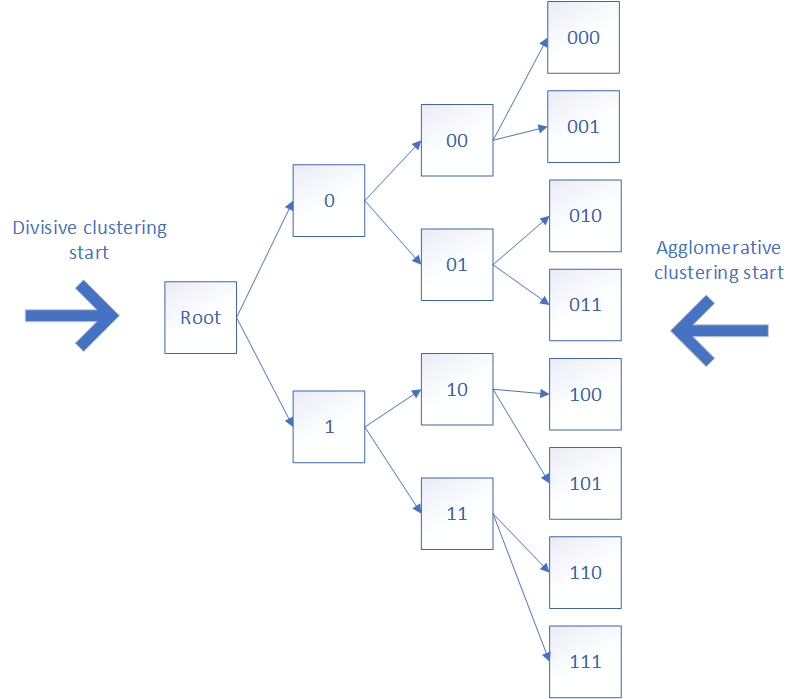
\includegraphics[width=.6\textwidth]{figures/clustering.png}
  \caption{Illustration of a data tree, arrows represent starting point for clustering process}
  \label{fig:clusterex}
\end{figure}

%Bottom-up vs top-down
Each method of hierarchical clustering has its advantages and disadvantages. 
The most significant problem for the Agglomerative clustering is the significant performance penalty that requires processing the dataset multiple times. 
Some variations of the method can improve on this performance drawback to some extent. 
However, in general, the performance penalty comes from the exhaustive search and checking every possibility of improvement on the resulting clusters. 
Divisive clustering solves the problem of performance penalties by starting with one big cluster that is split recursively into smaller clusters. 
The most significant drawback is the potential for more optimal clusters to be available in the sub-clusters, as these will not be checked for potential merges by the algorithm.

%Used in Springer article, describe the article, mention relevancy in passing
One example of agglomerative clustering used in the processing of audio samples is found in an article about a modified Dynamic Tree Warping method used in calculating distance between different audio samples\cite{ClusterExample}. 
The authors use agglomerative clustering to compare their modified DTW function with the standard, and then use two different scoring mechanisms to determine how well their function performed. 
The paper uses two different scoring mechanisms and both top out at around 15 to 20 clusters.
Results provided in this paper show potential diminishing results when using more than these numbers of clusters when processing audio.

%Section 4 on how both tie together somewhat, use Tree-CNN as base and work up the chain in references
\section{Neural networks and data clustering}
%What Tree-CNN is and what it did
The concept of using neural networks in tree structures is not new. 
As NN layers learn information in a structured manner that focuses on more generic feature detection in the first layers, expanding these networks to become more hierarchical classifiers is possible. 
One example of this is Tree-CNN \cite{roy2018treecnn}, which in addition to using multiple models in its solution, also implements incremental learning that expands the capability of the model over time, rather than training it on the entire dataset in one go.

The Tree-CNN paper sought to primarily resolve the problem of neural networks becoming final after their initial training. 
Once the training process is complete, the neural network cannot be generally re-purposed or modified to learn new information, at least not without losing critical information in the model that allowed it to perform well in its previous tasks. 
By using multiple models in a tree structure, more general classes were created in the root node of the tree that would classify multiple end classes as same, moving the complexity of determining the actual correct class to a more specialized branch node. 

In this particular paper, the branches were found to cluster classes in similar-looking groups, even if the classes were not too related to each other. 
More importantly, in the interest of this master thesis, table 6 of the paper describes the Tree-CNN as being relatively accurate while taking only 60\% of the time to construct. 

Another case of using data clustering in combination with CNNs is the HD-CNN paper\cite{hdcnn} from 2015.
The researchers in this paper used hierarchical clustering to cluster the image dataset into more coarse classes.
They then used information from those coarse classes in the later layers of the NN that were responsible for the fine classification into specific classes.
The top-k error results of HD-CNN were competitive with the first version of Inception\cite{szegedy2014going} and other models, beating them in some metrics.


%Figures:
%Small net figure - visio - done
%conv operation - visio?
%pooling operation - visio? - done
%MFCC sample graph - pull from spec report - done
%agg cluster picture - visio, arrows to point direction for explanation

